\section{Motivation}
\label{sec:CD+-kinetics-motivation}

This chapter will discuss the kinetics of the \CD molecular ion with neutral
helium atoms. The formation rate coefficient ($k_e$) for He$_n$\CD ($n$
indicates the number of He atoms attached to CD$^+$ ion) complexes are derived,
and their temperature dependence will be discussed. These kinetics measurements
are performed with and without the presence of radiation resonant with the \CD\
\CDline pure rotational transition via the ROSAA action spectroscopic technique
(see Section \ref{subsec:ROSAA} for more detail). The main motivation of these
studies is to understand the ROSAA process and its signal intensities in detail
with the support of numerical simulations. The \CD\ ion is best suited
for this purpose since at low collisional temperature ($<7$ K), one can
assume a two-level quantum system (Section
\ref{subsec:CD+-kinetics-simulation}) and state-dependent formation rate
coefficient $k_{e(J)}$ can be derived from a measured $k_e$, (Section
\ref{subsec:CD+-kinetics} and \ref{subsec:CD+-kinetics-simulation}) which can
provide us with an experimental comparison to the developed ROSAA numerical
model.

\section{Kinetics measurements}
\label{sec:CD+-kinetics}
The experiments were carried out using the 22-pole cryogenic ion trap instrument (FELion). A detailed account of the FELion instrument has been provided in Section \ref{sec:felion}. The \CD ions were produced by electron impact ionization (EI, electron energy $30-35$ eV) from a neutral CD$_4$ precursor (99 atoms \% D, Sigma-Aldrich). A short pulse, $\sim$50 ms, of mass-selected \CD (typically $\sim 10^4$ ions) is injected into the trap and stored for a specified time, typically $\sim 600-900$ ms for spectroscopic experiments, and varied between 0 and 6500 ms in $30-40$ steps for kinetic measurements, with continuous inflow of He buffer gas for collisional cooling and complex formation. By counting the primary \CD and He$_n$\CD complexes, and possibly other product ions formed by reactions with neutral contaminats, as a function of trap time, the association and collision-induced dissociation rate constants can be determined, which is discussed in Section \ref{subsec:rate-theory}. For measuring rotational transitions of \CD the ROSAA action spectroscopic technique is employed as described in Section \ref{subsec:ROSAA}. The pure-rotational spectra are measured in 10 kHz steps and are averaged over $\sim 20$ iterations.

\begin{figure}[!htb]

    \centering

    \begin{subfigure}[b]{0.49\textwidth}
        \centering
        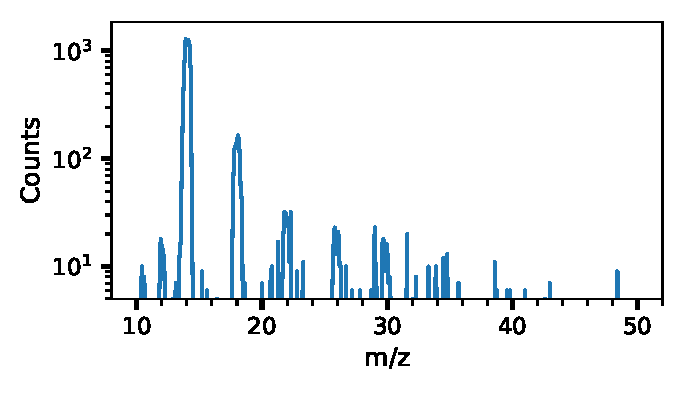
\includegraphics[width=1\textwidth]{figures/measurements/masspec/CD+_masspec_lowP_1.6e+14_4.8K.pdf}
        \caption{}
        \label{fig:masspec:lownHe}
    \end{subfigure}
    \hfill
    \begin{subfigure}[b]{0.49\textwidth}
        \centering
        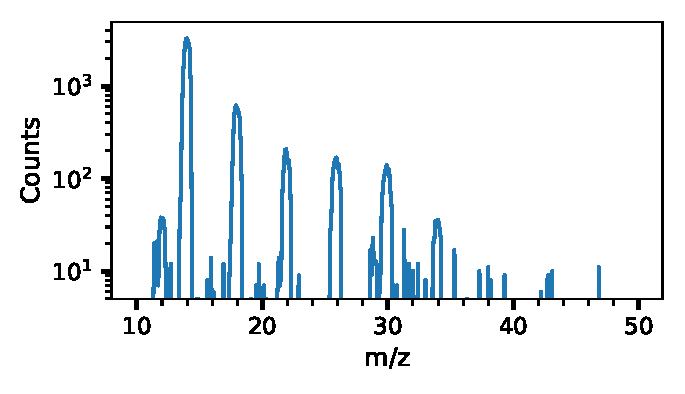
\includegraphics[width=1\textwidth]{figures/measurements/masspec/CD+_masspec_highP_2.5e+14_4.8K.pdf}
        \caption{}
        \label{fig:masspec:highnHe}
    \end{subfigure}
    
    \caption{ Measured mass spectrum after storing \CD ions (m/z $14$) for $\sim$600 ms in the cryogenic ion trap using He buffer gas (a): $1.97(7)\cdot10^{14}$~cm$^{-3}$; (b): $3.07(12)\cdot10^{14}$~cm$^{-3}$ number density at T=4.8(3)K, showing the \CD ion and the subsequent formation of ion-He complexes with up to (a): four; (b): five He atoms attached.}
    \label{fig:masspec}

\end{figure}


At low temperatures and high enough He number densities (typically $< 10$ K and
$> 1\cdot10^{14}$~cm$^{-3}$, respectively), the He$_n$CD$^+$ complexes are
readily formed by three-body collision processes but also dissociated by
collision-induced dissociation due to their low binding energies. The formation
and collisional dissociation processes of \CD + He are characterized by the
formation ($k_{e}$) and dissociation ($k_{CID}$) rate coefficients, discussed
in Sections \ref{subsec:rate-theory} and \ref{subsec:rate-equations}.

Figure \ref{fig:masspec} shows mass spectra of filtered and trapped \CD at
a nominal temperature $4.7(3)$ K. After storing \CD for about 600 ms, a 14(1)
$\%$ yield to attach the first He atom is achieved and up to two He atoms
(\ref{fig:masspec:lownHe}) are attached at $1.97(7) \cdot 10^{14}$ \percc.
Higher order complexes are formed by increasing the He number density as shown
in Figure \ref{fig:masspec:highnHe}, which also increases the He\CD yield. In
this study, the \CD + He kinetics measurements were performed for helium
number densities in the range of $1-7 \times 10^{14}$ \percc\ and in the 
$5 - 7$ K nominal trap temperature range.